\documentclass[10pt]{article}

\usepackage[margin=0.75in]{geometry}
\usepackage{amsmath,amsthm,amssymb,bm}
\usepackage{xcolor}
\usepackage{cancel}
\usepackage{graphicx}
\usepackage{changepage}
\usepackage{circuitikz}
\usepackage{pgfplots}
\usepackage{minted}
\usepackage{physics}
\usepackage{tikz}
\usepackage{tikz-3dplot}
\usepackage{hyperref}
\usepackage{siunitx}
\usepackage{fontspec}
\usepackage{relsize}
\usepackage{subfig}
\usepackage{todonotes}
\usepackage{contour}
\usepackage{multicol, multirow, booktabs}
\usepackage[breakable]{tcolorbox}
\usepackage[inline]{enumitem}

\theoremstyle{definition}
\newtheorem{problem}{Problem}
\newtheorem{soln}{Solution}

\pgfplotsset{compat=newest}
\usetikzlibrary{lindenmayersystems}
\usetikzlibrary{arrows}
\usetikzlibrary{calc}
\usetikzlibrary{positioning, fit}
\usetikzlibrary{3d, perspective}
\usetikzlibrary{math}
\usetikzlibrary{fadings}
\usetikzlibrary{angles,quotes} 
\usetikzlibrary{decorations.markings}

\definecolor{incolor}{HTML}{303F9F}
\definecolor{outcolor}{HTML}{D84315}
\definecolor{cellborder}{HTML}{CFCFCF}
\definecolor{cellbackground}{HTML}{F7F7F7}
\newcommand{\ui}{\hat{i}}
\newcommand{\uj}{\hat{j}}
\newcommand{\uk}{\hat{k}}
\newcommand{\ux}{\hat{\mathbf{x}}}
\newcommand{\uy}{\hat{\mathbf{y}}}
\newcommand{\uz}{\hat{\mathbf{z}}}
\newcommand{\uv}[1]{\hat{\bv{{#1}}}}
\newcommand{\pr}[1]{{#1^\prime}}
\newcommand{\pd}[2][]{{\frac{\partial^{#1}}{\partial {{#2}^{#1}}}}}
\newcommand{\dif}[2][]{{\frac{d^{#1}}{d{{#2}^{#1}}}}}
\newcommand{\grd}{\nabla}

\pgfdeclarelayer{background}  
\pgfsetlayers{background,main}
\AtBeginDocument{\RenewCommandCopy\qty\SI}

\makeatletter
\newcommand{\boxspacing}{\kern\kvtcb@left@rule\kern\kvtcb@boxsep}
\makeatother
\newcommand{\prompt}[4]{
    \ttfamily\llap{{\color{#2}[#3]:\hspace{3pt}#4}}\vspace{-\baselineskip}
}

\newcommand{\thevenin}[2]{
  \begin{center}
    \begin{circuitikz} \draw
      (0,0) -- (2,0) to[battery1, l_=$V_{Th}\eq#1$] (2,2) 
      to[resistor, l_=$R_{Th}\eq#2$] (0,2)
      ;
      \draw [o-] (-.07,2.079);
      \draw [o-] (-.07,0.079);
    \end{circuitikz}
  \end{center}
}

\newcommand{\norton}[2]{
  \begin{center}
    \begin{circuitikz} \draw
      (0,0) -- (3,0) to[american current source, l_=$I_{N}\eq#1$] (3,2) -- (0,2) (2,0)
      to[resistor, l=$R_{N}\eq#2$] (2,2)
      ;
      \draw [o-] (-.07,2.079);
      \draw [o-] (-.07,0.079);
    \end{circuitikz}
  \end{center}
}

\DeclareMathOperator{\Div}{div}
\DeclareMathOperator{\Curl}{curl}
\DeclareMathOperator{\sgn}{sgn}

\newcommand{\highlight}[1]{\colorbox{yellow}{$\displaystyle #1$}}
\newcommand{\ti}[1]{\widetilde{#1}}
\renewcommand{\div}[1]{\bv{\nabla}\cdot #1}
\renewcommand{\curl}[1]{\bv{\nabla}\times #1}

\newfontface{\Kaufmann}{Kaufmann}
\DeclareTextFontCommand{\kf}{\Kaufmann}
\newcommand{\scriptr}{\fontsize{12pt}{12pt}\kf{r}\fontsize{10pt}{10pt}}

\newfontface{\KaufmannB}{Kaufmann Bold}
\DeclareTextFontCommand{\kfb}{\KaufmannB}
\newcommand{\bscriptr}{\fontsize{12pt}{12pt}\kfb{r}\fontsize{10pt}{10pt}}
\newcommand{\justif}[2]{&{#1}&\text{#2}}
\newcommand{\bv}[1]{\bm{\mathrm{#1}}}

\title{Physics 4240H: Assignment I}
\author{Jeremy Favro (0805980) \\ Trent University, Peterborough, ON, Canada}
\date{\today}

\begin{document}
\maketitle

% PROBLEM 1
\begin{problem}[4.2]
A transverse wave pulse, described by
$$y=\frac{4}{x^2+2}$$
is initiated at $t=0$ in a stretched string, where all values are given in SI units.
\begin{enumerate}[label=(\alph*)]
  \item Write an expression describing the disturbance $y(x,t)$ in the traveling pulse as a function of time, $t$, and position,
        $x$, if it moves with a speed of $\qty{3.7}{\meter\per\second}$ in the negative $x$-direction.
  \item Plot the pulse at $t=0$, $t=2$, and $=\qty{5}{\second}$.
\end{enumerate}
\end{problem}
\begin{soln}~
  \begin{enumerate}[label=(\alph*)]
    \item $$y(x,t)=\frac{4}{(x+3.7t)^2+2}.$$ The plus sign on the velocity accounts for the $-x$ propagation.
    \item ~\begin{center}
            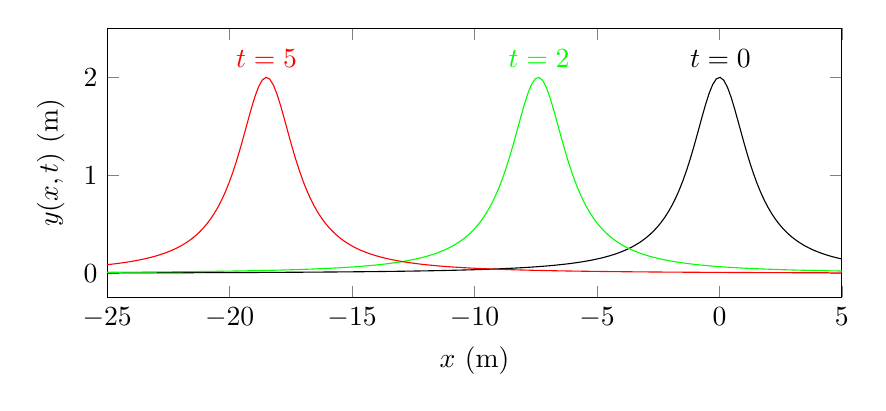
\begin{tikzpicture}
              \begin{axis}[
                  width=\textwidth*0.9, height = 5cm,
                  xlabel={$x$ (m)}, ylabel={$y(x,t)$ (m)},
                  xmin=-25, xmax=5, ymax=2.5
                ]
                \addplot[domain=-25:5, samples=200, color=black](\x,{4/((x)^2+2)}) node[pos=0.824, above]{$t=0$};
                \addplot[domain=-25:5, samples=200, color=green](\x,{4/((x+3.7*2)^2+2)}) node[pos=0.585, above]{$t=2$};
                \addplot[domain=-25:5, samples=200, color=red](\x,{4/((x+3.7*5)^2+2)}) node[pos=0.226, above]{$t=5$};
              \end{axis}
            \end{tikzpicture}
          \end{center}
  \end{enumerate}
\end{soln}

% PROBLEM 2
\begin{problem}[4.5]
A harmonic traveling wave is moving in the negative $z$-direction with amplitude 2 (in arbitrary units), wavelength $\qty{5}{\meter}$, and period $\qty{3}{\second}$.
Its disturbance at the origin is a maximum at time zero. Using the cosine form of a harmonic wave, write an expression for this wave with all values in SI units:
\begin{enumerate}[label=(\alph*)]
  \item that exhibits directly wavelength and period;
  \item that exhibits directly both the propagation constant and velocity;
  \item in complex form.
\end{enumerate}
\end{problem}
\begin{soln}
  \begin{enumerate}[label=(\alph*)]
    \item $y(x,t)=2\cos(\frac{2\pi}{\qty{5}{\meter}}z+\frac{2\pi}{\qty{3}{\second}}t)$.
    \item $y(x,t)=2\cos(\frac{2\pi}{\qty{5}{\meter}}\left[z+\frac{\qty{5}{\meter}}{\qty{3}{\second}}t\right])$.
    \item Not sure if you want the cosine in complex form or just an exponential. I'll assume exponential because it's easy to get the real part out of that later,
          $y(x,t)=2\exp(i(\frac{2\pi}{\qty{5}{\meter}}z+\frac{2\pi}{\qty{3}{\second}}t))$.
  \end{enumerate}
\end{soln}

% PROBLEM 3
\begin{problem}[4.11]
By finding the appropriate expressions for $\bv{k}\cdot\bv{r}$, write expressions for a harmonic plane wave in three dimensions (you may assume the initial phase is zero),
displaying wavelength and velocity, if the propagation is:
\begin{enumerate}[label=(\alph*)]
  \item along the $+z$-axis;
  \item along the line $x=y$, $z=0$;
  \item perpendicular to the plane $x+y+z=\mathrm{constant}$.
\end{enumerate}
\end{problem}
\begin{soln}
  \begin{enumerate}[label=(\alph*)]
    \item $\exp(i(\frac{2\pi}{\lambda}z-vt))$. Here $\bv{k}=\frac{2\pi}{\lambda}\uz$, $\bv{r}=z\uz$.
    \item $\exp(i(\frac{2\pi}{\sqrt{2}\lambda}\left[x+y\right]-vt))$. Here $\bv{k}=\frac{2\pi}{\sqrt{2}\lambda}\left[\ux+\uy\right]$, $\bv{r}=x\ux+y\uy$.
    \item $\exp(i(\frac{6\pi}{\sqrt{2}\lambda}\left[x+y+z\right]-vt))$. Here $\bv{k}=\frac{6\pi}{\sqrt{2}\lambda}\left[\ux+\uy+\uz\right]$, $\bv{r}=x\ux+y\uy+z\uz$.
  \end{enumerate}
\end{soln}

% PROBLEM 4
\begin{problem}[4.24]
Consider the electric field
$$\bv{E}=E_{0x}\cos(kz-\omega t +\phi_{0x})\ux+E_{0y}\cos(kz-\omega t +\phi_{0y}).$$
Produce plots like those in Figure 4.11 that show the evolution of the electric field vector, in the plane $z=0$, as a function of time over one complete period for the following
cases:
\begin{enumerate}[label=(\alph*)]
  \item $E_{0x}=2E_{0y};\phi_{0x}=\phi_{0y}=0$
  \item $E_{0x}=2E_{0y};\phi_{0x}=0;\phi_{0y}=\pi/2$
  \item $E_{0x}=2E_{0y};\phi_{0x}=0;\phi_{0y}=-\pi/2$
  \item $E_{0x}=2E_{0y};\phi_{0x}=\pi/4;\phi_{0y}=-\pi/4$
  \item $E_{0x}=2E_{0y};\phi_{0x}=0;\phi_{0y}=-\pi/4$
\end{enumerate}
\end{problem}

\begin{soln}~
  \begin{enumerate}[label=(\alph*)]
    \item ~\begin{center}
            \foreach \t in {0,...,5}{
                \begin{tikzpicture}
                  \tikzset{>=latex}
                  \tikzstyle{vector}=[-stealth,red!90!black,thick,line cap=round]

                  % CONSTANTS
                  \def\mrvec{2}
                  \def\omga{3*3.14159/2}
                  \def\phix{0}
                  \def\phiy{0}

                  \coordinate (O) at (0,0);
                  \draw[thick,->] (-\mrvec,0) -- (\mrvec,0) node[anchor=north east]{$x$};
                  \draw[thick,->] (0,-\mrvec) -- (0,\mrvec) node[anchor=north west]{$y$};

                  \draw[vector] (O) -- ({2*cos(deg(-\omga*\t+\phix))},{cos(deg(-\omga*\t+\phiy))});
                  \node[] at (\mrvec, \mrvec) {$\bv{E}(t=\t)$};
                \end{tikzpicture}
              }
          \end{center}
    \item ~\begin{center}
            \foreach \t in {0,...,5}{
                \begin{tikzpicture}
                  \tikzset{>=latex}
                  \tikzstyle{vector}=[-stealth,red!90!black,thick,line cap=round]

                  % CONSTANTS
                  \def\mrvec{2}
                  \def\omga{3*3.14159/2}
                  \def\phix{0}
                  \def\phiy{3.14159/2}

                  \coordinate (O) at (0,0);
                  \draw[thick,->] (-\mrvec,0) -- (\mrvec,0) node[anchor=north east]{$x$};
                  \draw[thick,->] (0,-\mrvec) -- (0,\mrvec) node[anchor=north west]{$y$};

                  \draw[vector] (O) -- ({2*cos(deg(-\omga*\t+\phix))},{cos(deg(-\omga*\t+\phiy))});
                  \node[] at (\mrvec, \mrvec) {$\bv{E}(t=\t)$};
                \end{tikzpicture}
              }
          \end{center}
    \item ~\begin{center}
            \foreach \t in {0,...,5}{
                \begin{tikzpicture}
                  \tikzset{>=latex}
                  \tikzstyle{vector}=[-stealth,red!90!black,thick,line cap=round]

                  % CONSTANTS
                  \def\mrvec{2}
                  \def\omga{3*3.14159/2}
                  \def\phix{0}
                  \def\phiy{-3.14159/2}

                  \coordinate (O) at (0,0);
                  \draw[thick,->] (-\mrvec,0) -- (\mrvec,0) node[anchor=north east]{$x$};
                  \draw[thick,->] (0,-\mrvec) -- (0,\mrvec) node[anchor=north west]{$y$};

                  \draw[vector] (O) -- ({2*cos(deg(-\omga*\t+\phix))},{cos(deg(-\omga*\t+\phiy))});
                  \node[] at (\mrvec, \mrvec) {$\bv{E}(t=\t)$};
                \end{tikzpicture}
              }
          \end{center}
    \item ~\begin{center}
            \foreach \t in {0,...,5}{
                \begin{tikzpicture}
                  \tikzset{>=latex}
                  \tikzstyle{vector}=[-stealth,red!90!black,thick,line cap=round]

                  % CONSTANTS
                  \def\mrvec{2}
                  \def\omga{3*3.14159/2}
                  \def\phix{3.14159/4}
                  \def\phiy{-3.14159/4}

                  \coordinate (O) at (0,0);
                  \draw[thick,->] (-\mrvec,0) -- (\mrvec,0) node[anchor=north east]{$x$};
                  \draw[thick,->] (0,-\mrvec) -- (0,\mrvec) node[anchor=north west]{$y$};

                  \draw[vector] (O) -- ({2*cos(deg(-\omga*\t+\phix))},{cos(deg(-\omga*\t+\phiy))});
                  \node[] at (\mrvec, \mrvec) {$\bv{E}(t=\t)$};
                \end{tikzpicture}
              }
          \end{center}
    \item ~\begin{center}
            \foreach \t in {0,...,5}{
                \begin{tikzpicture}
                  \tikzset{>=latex}
                  \tikzstyle{vector}=[-stealth,red!90!black,thick,line cap=round]

                  % CONSTANTS
                  \def\mrvec{2}
                  \def\omga{3*3.14159/2}
                  \def\phix{0}
                  \def\phiy{-3.14159/4}

                  \coordinate (O) at (0,0);
                  \draw[thick,->] (-\mrvec,0) -- (\mrvec,0) node[anchor=north east]{$x$};
                  \draw[thick,->] (0,-\mrvec) -- (0,\mrvec) node[anchor=north west]{$y$};

                  \draw[vector] (O) -- ({2*cos(deg(-\omga*\t+\phix))},{cos(deg(-\omga*\t+\phiy))});
                  \node[] at (\mrvec, \mrvec) {$\bv{E}(t=\t)$};
                \end{tikzpicture}
              }
          \end{center}
  \end{enumerate}

\end{soln}


% PROBLEM 5
\begin{problem}
Explore Interactive Animation 4.2 and determine from writing down the results from moving the sliders the amplitude, propagation constant, period, and initial phase of the wave.
\end{problem}
\begin{soln}
  The amplitude is easy enough, the wave is bounded between $\pm1$ so it has amplitude 1. The propagation constant, $k=2\pi/\lambda$ we can kind of guess at by finding the wavelength.
  Looking at the first figure, the slider snaps at $y(1.5,1)=-0.5$ and $y=(3,1)=-0.5$, a full cycle. This gives a wavelength of
  $\lambda=1.5$ and hence $k=2\pi/1.5=4\pi/3$. Looking at the bottom figure for the period we use the same strategy and look at
  $y(1,2)=-0.5$ and $y(1,3.5)=-0.5$, another full cycle. This gives a period of $\qty{1.5}{\second}$. To determine the initial phase we have to
  assume that the wave is a cosine. If this is the case, at $y(1,1)=\cos(\frac{8\pi}{3}+\phi)=1\implies\phi=-8\pi/3$. In effect this is the same as an
  initial phase of $2\pi/3$ as we can just add $2\pi$ twice.
\end{soln}

% PROBLEM 6
\begin{problem}
A linearly polarized electromagnetic wave travels in the $+x$-direction in dry air. The amplitude of the electric field is $\qty{1.52}{\volt\per\meter}$,
the frequency of the wave is $\qty{520}{\tera\hertz}$, and the precise direction of the polarization is unspecified (although you may assume that the initial
phase of both components is zero).
\begin{enumerate}[label=(\roman*)]
  \item With all values in SI units, what is the best scalar representation (I'm not repeating all the choices) of the electric field of the wave.
  \item If the wave is discovered to be linearly polarized along the $y$-axis, then in SI units which of the following expressions, containing 
  the wavelength $\lambda$ and period $T$, is the best representation of the \emph{magnetic field} of the wave?
  \item The wave travels into a glass slab with front surface perpendicular to the direction of travel, in the $yz$-plane. The speed of the wave 
  within the glass is $\qty{2.17e8}{\meter\per\second}$. Which of the following forms best represents the transmitted electric field of the wave 
  inside the glass, with amplitude $E_0$?
  \item The slab of glass is now rotated about an axis parallel to the $z$-axis, so that the \emph{front face} of the glass makes an angle
  with the $x$-axis of $\qty{30}{\degree}$. Which of the following propagation vectors now best describes the direction of propagation of the transmitted
  wave in the glass?
\end{enumerate}
\end{problem}
\begin{soln}~
\begin{enumerate}[label=(\roman*)]
  \item We are directly given the amplitude. Since the wave is traveling in $+\ux$ the sign on the time term ought to be negative. Then we just have to find
  $k=2\pi/\lambda=2\pi/(c_0/\nu)\approx \qty{1.09e7}{\per\meter}$. We could calculate the angular frequency to confirm but this is sufficient to 
  narrow the answer down to (A).
  \item Since the wave as a whole is propagating in $+\ux$ the $B$-field must be in the $xz$-plane if the $E$-field is to be in the $yx$-plane. Additionally,
  since the wave is propagating along $\ux$ it ought to depend on $x$ and $t$ only, so the only acceptable answer is (E).
  \item Since the light slows down its wavelength must decrease to maintain frequency (and thereby boundary continuity is the way I understand it).
  This means that since $\nu =c/\lambda$ and $c$ has decreased in the glass, $\lambda$ must also decrease. This means we expect $k$ to increase.
  We don't expect that $E$ will change in polarization so we can, using these two, knock out (B) \& (E) as they are in $\uz$ and 
  (D) as $k$ hasn't changed. To select between (A) and (C) we recall that $\omega=2\pi\nu$ and $\nu$, the frequency, remains the same so (A)
  has to be correct as it has the same $\omega$ as (i).
  \item I wanted to do this with Snell's law at first but since it wasn't in this chapter I wasn't sure about that. The way the answers are written,
  splitting the magnitude and direction, gave me the thought to check magnitudes. The only one close to being normalized is (B), so that is my answer.
\end{enumerate}
\end{soln}
\end{document}